

\section{Evaluation of features}
\label{sec:evaluation-of-features}

\subsection{JIT - Just In Time Compilation}
\label{sec:jit}

\subsection{Interpreter}
\label{sec:interpreter}

\subsection{WASM to native compilation}
\label{sec:wasm-to-native}

\subsection{AOT - Ahead Of Time Compilation}
\label{sec:aot}


 \subsection{Javascript snapshotting (Wizer)}
\label{sec:wizer}

\section{Comparison to V8 Isolates}
\label{sec:v8-comparison}
A V8 isolate is a separate instance of the V8 engine that has its own memory, garbage collector, and global object \cite{a2021_isolate}. An isolate can run scripts in a safe and isolated environment, without interfering with other isolates \cite{cloudflareinc_2023_how}. An isolate also has its own state, which means that objects from one isolate cannot be used in another isolate. When V8 is initialized, a default isolate is created and entered, but you can also create your own isolates using the V8 API \cite{a2021_isolate}.

\begin{figure}[htbp]
	\centering
		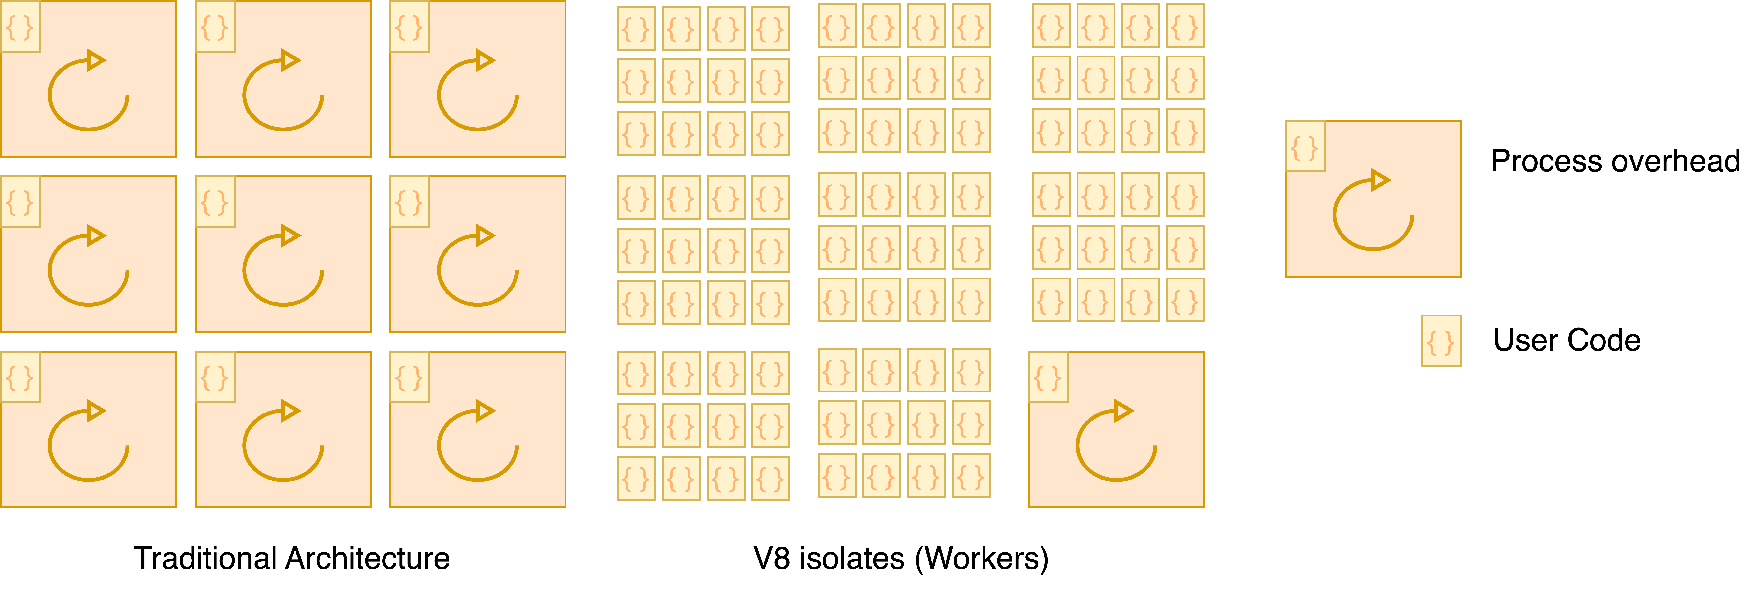
\includegraphics[width=\textwidth,height=\textheight,keepaspectratio]{images/runtimes/v8-isolates.pdf}
	\caption{containerized vs. \gls{V8} \glspl{isolate} figure redrawn from \cite{cloudflareinc_2023_how}}
	\label{fig:v8-isolates}
\end{figure}

\subsection{Advantages and disadvantages}
\label{sec:advantages-disadvantages}